\documentclass[]{article}
\usepackage{lmodern}
\usepackage{amssymb,amsmath}
\usepackage{ifxetex,ifluatex}
\usepackage{fixltx2e} % provides \textsubscript
\ifnum 0\ifxetex 1\fi\ifluatex 1\fi=0 % if pdftex
  \usepackage[T1]{fontenc}
  \usepackage[utf8]{inputenc}
\else % if luatex or xelatex
  \ifxetex
    \usepackage{mathspec}
  \else
    \usepackage{fontspec}
  \fi
  \defaultfontfeatures{Ligatures=TeX,Scale=MatchLowercase}
\fi
% use upquote if available, for straight quotes in verbatim environments
\IfFileExists{upquote.sty}{\usepackage{upquote}}{}
% use microtype if available
\IfFileExists{microtype.sty}{%
\usepackage[]{microtype}
\UseMicrotypeSet[protrusion]{basicmath} % disable protrusion for tt fonts
}{}
\PassOptionsToPackage{hyphens}{url} % url is loaded by hyperref
\usepackage[unicode=true]{hyperref}
\hypersetup{
            pdftitle={Final Report},
            pdfauthor={Nick Mandarano and Patrick McHugh},
            pdfborder={0 0 0},
            breaklinks=true}
\urlstyle{same}  % don't use monospace font for urls
\usepackage[margin=1in]{geometry}
\usepackage{color}
\usepackage{fancyvrb}
\newcommand{\VerbBar}{|}
\newcommand{\VERB}{\Verb[commandchars=\\\{\}]}
\DefineVerbatimEnvironment{Highlighting}{Verbatim}{commandchars=\\\{\}}
% Add ',fontsize=\small' for more characters per line
\usepackage{framed}
\definecolor{shadecolor}{RGB}{248,248,248}
\newenvironment{Shaded}{\begin{snugshade}}{\end{snugshade}}
\newcommand{\KeywordTok}[1]{\textcolor[rgb]{0.13,0.29,0.53}{\textbf{#1}}}
\newcommand{\DataTypeTok}[1]{\textcolor[rgb]{0.13,0.29,0.53}{#1}}
\newcommand{\DecValTok}[1]{\textcolor[rgb]{0.00,0.00,0.81}{#1}}
\newcommand{\BaseNTok}[1]{\textcolor[rgb]{0.00,0.00,0.81}{#1}}
\newcommand{\FloatTok}[1]{\textcolor[rgb]{0.00,0.00,0.81}{#1}}
\newcommand{\ConstantTok}[1]{\textcolor[rgb]{0.00,0.00,0.00}{#1}}
\newcommand{\CharTok}[1]{\textcolor[rgb]{0.31,0.60,0.02}{#1}}
\newcommand{\SpecialCharTok}[1]{\textcolor[rgb]{0.00,0.00,0.00}{#1}}
\newcommand{\StringTok}[1]{\textcolor[rgb]{0.31,0.60,0.02}{#1}}
\newcommand{\VerbatimStringTok}[1]{\textcolor[rgb]{0.31,0.60,0.02}{#1}}
\newcommand{\SpecialStringTok}[1]{\textcolor[rgb]{0.31,0.60,0.02}{#1}}
\newcommand{\ImportTok}[1]{#1}
\newcommand{\CommentTok}[1]{\textcolor[rgb]{0.56,0.35,0.01}{\textit{#1}}}
\newcommand{\DocumentationTok}[1]{\textcolor[rgb]{0.56,0.35,0.01}{\textbf{\textit{#1}}}}
\newcommand{\AnnotationTok}[1]{\textcolor[rgb]{0.56,0.35,0.01}{\textbf{\textit{#1}}}}
\newcommand{\CommentVarTok}[1]{\textcolor[rgb]{0.56,0.35,0.01}{\textbf{\textit{#1}}}}
\newcommand{\OtherTok}[1]{\textcolor[rgb]{0.56,0.35,0.01}{#1}}
\newcommand{\FunctionTok}[1]{\textcolor[rgb]{0.00,0.00,0.00}{#1}}
\newcommand{\VariableTok}[1]{\textcolor[rgb]{0.00,0.00,0.00}{#1}}
\newcommand{\ControlFlowTok}[1]{\textcolor[rgb]{0.13,0.29,0.53}{\textbf{#1}}}
\newcommand{\OperatorTok}[1]{\textcolor[rgb]{0.81,0.36,0.00}{\textbf{#1}}}
\newcommand{\BuiltInTok}[1]{#1}
\newcommand{\ExtensionTok}[1]{#1}
\newcommand{\PreprocessorTok}[1]{\textcolor[rgb]{0.56,0.35,0.01}{\textit{#1}}}
\newcommand{\AttributeTok}[1]{\textcolor[rgb]{0.77,0.63,0.00}{#1}}
\newcommand{\RegionMarkerTok}[1]{#1}
\newcommand{\InformationTok}[1]{\textcolor[rgb]{0.56,0.35,0.01}{\textbf{\textit{#1}}}}
\newcommand{\WarningTok}[1]{\textcolor[rgb]{0.56,0.35,0.01}{\textbf{\textit{#1}}}}
\newcommand{\AlertTok}[1]{\textcolor[rgb]{0.94,0.16,0.16}{#1}}
\newcommand{\ErrorTok}[1]{\textcolor[rgb]{0.64,0.00,0.00}{\textbf{#1}}}
\newcommand{\NormalTok}[1]{#1}
\usepackage{graphicx,grffile}
\makeatletter
\def\maxwidth{\ifdim\Gin@nat@width>\linewidth\linewidth\else\Gin@nat@width\fi}
\def\maxheight{\ifdim\Gin@nat@height>\textheight\textheight\else\Gin@nat@height\fi}
\makeatother
% Scale images if necessary, so that they will not overflow the page
% margins by default, and it is still possible to overwrite the defaults
% using explicit options in \includegraphics[width, height, ...]{}
\setkeys{Gin}{width=\maxwidth,height=\maxheight,keepaspectratio}
\IfFileExists{parskip.sty}{%
\usepackage{parskip}
}{% else
\setlength{\parindent}{0pt}
\setlength{\parskip}{6pt plus 2pt minus 1pt}
}
\setlength{\emergencystretch}{3em}  % prevent overfull lines
\providecommand{\tightlist}{%
  \setlength{\itemsep}{0pt}\setlength{\parskip}{0pt}}
\setcounter{secnumdepth}{0}
% Redefines (sub)paragraphs to behave more like sections
\ifx\paragraph\undefined\else
\let\oldparagraph\paragraph
\renewcommand{\paragraph}[1]{\oldparagraph{#1}\mbox{}}
\fi
\ifx\subparagraph\undefined\else
\let\oldsubparagraph\subparagraph
\renewcommand{\subparagraph}[1]{\oldsubparagraph{#1}\mbox{}}
\fi

% set default figure placement to htbp
\makeatletter
\def\fps@figure{htbp}
\makeatother


\title{Final Report}
\author{Nick Mandarano and Patrick McHugh}
\date{4/26/2022}

\begin{document}
\maketitle

\subsection{Introduction}\label{introduction}

To recap our proposal, we chose to do an NBA-related project and decided
to fit a regression model for salary of NBA players, using statistics
and other information about the players as covariates.

Our data includes many seasonal statistics for each player, including
both simple stats and advanced metrics. We also have access to other
personal information for each player, such as team, position, height,
etc.

We are modeling based on the 2015-16 NBA season. We know salary is known
before the season starts and statistics are created, so it is not a
response variable in the traditional sense of a causal effect. We
attempt to explore the relationship between salary and the covariates,
and aim to prescribe a true mean function, and identify players who may
be overperforming or underperforming their contract according to the
2015-16 market; i.e., putting up better or worse statistics than one
might expect a player on their salary to do.

\subsection{Data Exploration}\label{data-exploration}

Our data comes from four different datasets. We used three of Riguang
Wen's
\href{https://figshare.com/articles/dataset/NBA_data/5414170}{datasets}
from figshare.com -- \texttt{players cv}, \texttt{players salary}, and
\texttt{players stat}. We also used a
\href{https://zenodo.org/record/3750329\#.YkT6YW7MJAe}{dataset} called
\texttt{NBA RS 2020-1950 Stats} uploaded to zenodo.org by Pablo Gomez
and Sandra Giral.

In addition to player salary, the data available to us included
statistics from each player for the season, including basic stats such
as games played, points, and steals, as well as advanced stats such as
Value Over Replacement Player (VORP), Defensive Box +/- (DBPM), and
others. Other information included personal and demographic data related
to the players, such as age, height, college attended, birthplace, and
other things. A full list of variables can be found in the previously
submitted EDA description.

We proceeded to filter out players who were below the league minimum in
salary, as they were exclusively players signed to short term (i.e.,
10-day) contracts with wildly volatile data. We felt that players on
shorter than full season contracts would be worth creating a separate
model for in another project.

From our EDA, we concluded that a log transformation of the response
variable, salary, would be appropriate based on its skewed distribution.

We also noticed that many of the covariates had skewed distributions, or
did not have linear marginal relationships with the response variable
log(salary). We attempted to make these variables approximately normally
distirbutied with an approximately linear marginal relationship with the
response. We experimented with log, square root, and squaring
transformations. In the end, we consider the following transformations
in our model:

\begin{itemize}
\tightlist
\item
  VORP: A min/max normalization between 0 and 1 to eliminate negative
  values; then a log transformation
\item
  OWS: A min/max normalization between 0 and 1 to eliminate negative
  values; then a log transformation
\item
  DWS: Square root transformation
\item
  PTS: Square root transformation
\item
  FTr: Square root transformation
\item
  BLK: Log transformation
\item
  STL: Log transformation
\item
  GS: Log transformation
\item
  ORB: Log transformation
\end{itemize}

We use VORP as an example in the appendix. Figure A1 shows the
distribution of VORP and its plot against log(salary) both pre- and
post-transformation. Though not perfect, the transformed variable
appears to be much more appropriate for a linear model than the raw
variable.

We can also see that Pos has some redundancy and maybe too much
granularity. For example, ``F-C'' (forward/center) and ``C-F''
(center/forward) are treated as different positions by the model when
they are functionally the same. We cleaned this up by grouping players
into ``Guards'', ``Wings'', and ``Bigs'' according to Pos. Figure A2
shows this variable pre- and post-transformation. From the graph, it is
unclear if there is a significant relationship between the refined
position predictor Pos\_cat and log(salary).

We modified some other categorical variables as well. Over several
iterations of model building, we were able to reduce the Team variable
to a simple flag, Multiteam. A player appearing with multiple teams over
the course of the season had a strong relationship with salary.

Once our predictors are appropriately transformed, we considered all
pairwise correlations between continuous covariates as an initial search
for possibly collinearity, which we will discuss in more detail later.

\subsection{Variable Selection}\label{variable-selection}

Three pairs of predictors with noticably large correlations according
the the correlation matrix are further investigated. We learn that
pts\_adj and MP have a correlation coefficient of \(0.947\), ORtg and
TS. have a correlation coefficient of \(0.888\), and finally WS.48 and
PER have a correlation coefficient of \(0.864\). To avoid redundancy in
the model, we'll remove one predictor in each of the three pairs from
the model. The terms' variance inflation factors will guide the decision
regarding which predictor to drop. Using GVIF\(^\frac{1}{2df}\) will
allow the GVIFs to be comparable across dimensions. Thus, we remove
pts\_adj (8.77 \textgreater{} 6.25), TS. (4.64 \textgreater{} 4.29), and
WS.48 (8.42 \textgreater{} 7.42).

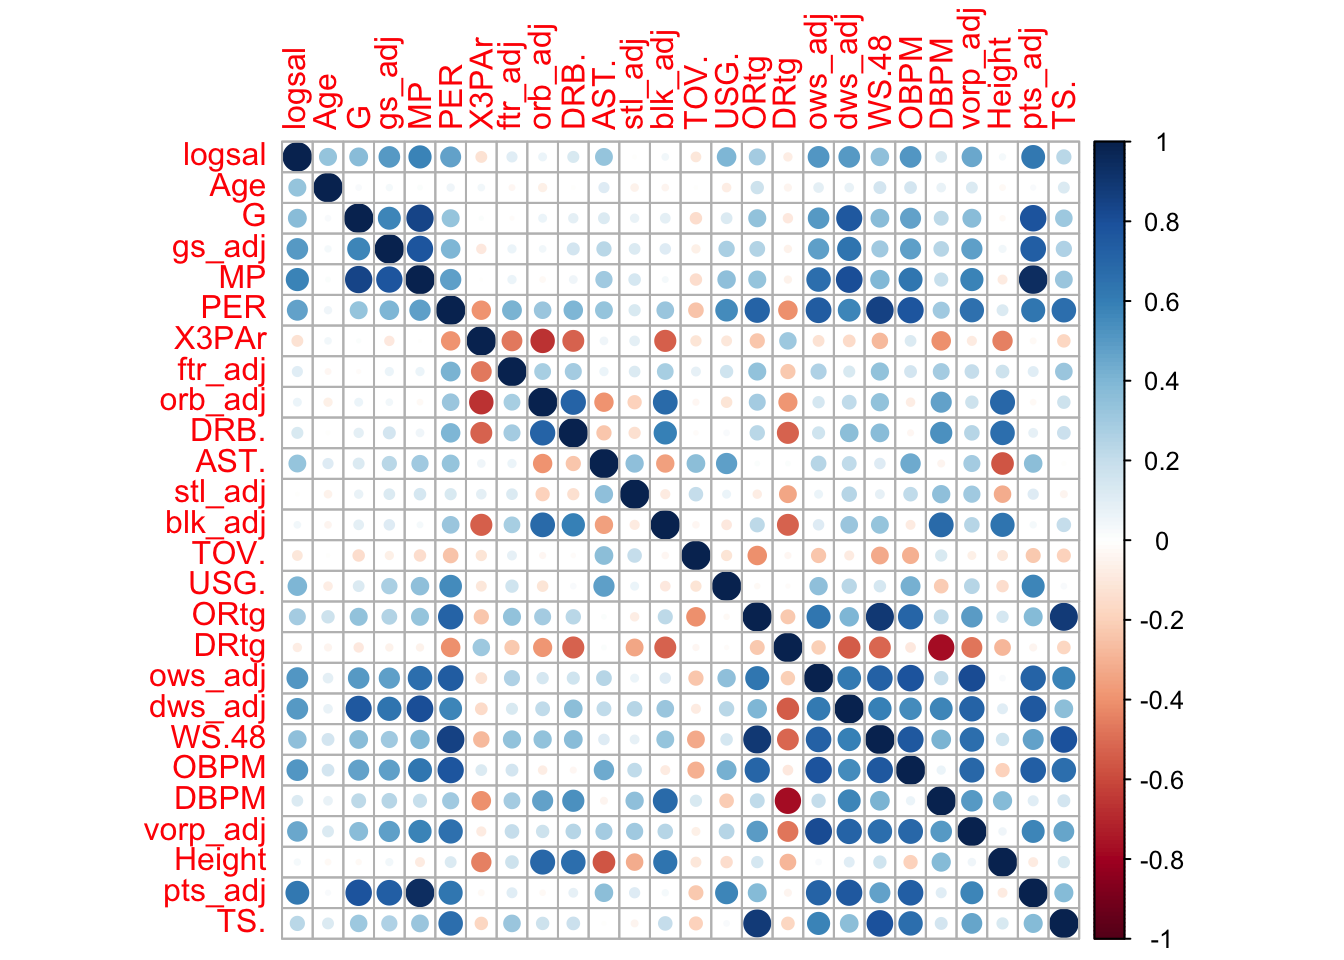
\includegraphics{FinalReportNew_files/figure-latex/unnamed-chunk-2-1.pdf}

We will begin by looking at a full model with all remaining predictors
and employ stepwise regression methods to find the best model. According
to BIC, the stepwise regression model working in both directions returns
MP, Age, USG., G and orb\_adj as predictors. We'll call this Model A.
The model using AIC in its variable selection process additionally
returns AST., stl\_adj, Pos\_cat, Multiteam, and TOV.. We'll call this
Model B.

Interactions of predictors may also be of interest in our model.
Intuitively, it would make sense if the effect of offensive rebounds on
a player's salary was dependent on the player's position. Therefore,
we'll also consider models with interaction terms, but with 26 possible
main effects, there are at least \(26(25)=650\) possible interaction
terms. We'll use the regsubsets function in the leaps package to return
the best models of each size, setting a conservative limit of the number
of variables in the model to 50.

\begin{verbatim}
## Reordering variables and trying again:
\end{verbatim}

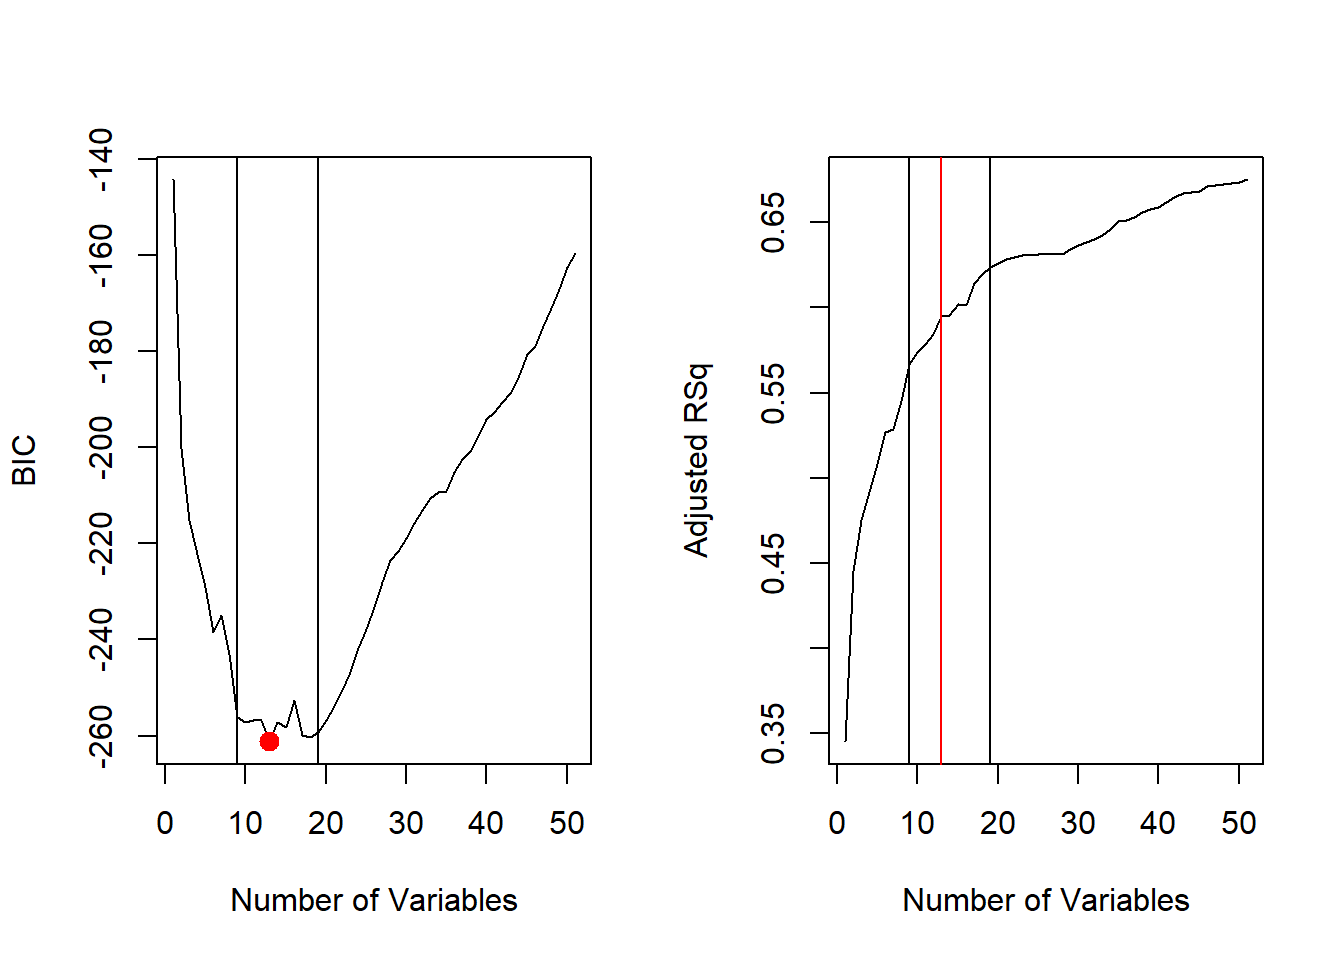
\includegraphics{FinalReportNew_files/figure-latex/unnamed-chunk-3-1.pdf}

Of these best models previously mentioned, we see that the model with
the smallest BIC is the best model chosen with 13 variables. Though the
Adjusted \(R^2\) of a model does not necessarily have to increase as
more variables are added, we see that in this case, the Adjusted \(R^2\)
is non-decreasing in the number of variables at least up to 50.
Practically, a model with 50 variables is not ideal. There seems to be a
point in the Adjusted \(R^2\) plot in which the rate of change begins to
flatten out that matches well with the point in the BIC plot where the
BIC begins to rise again. This point is the best model chosen with 19
variables. Similarly, the best model chosen with 9 variables corresponds
to an appropriate lower bound for the number of variables with both a
satisfactory BIC and Adjusted \(R^2\).

As we continued the model building process, we wanted to make sure we
were avoiding overfitting. We created an algorithm where we used the
regsubsets function to identify the n best predictors for all n from 1
to a large number, and included first level interaction effects. While
some of these models included interactions without the corresponding
main effects, we just used this as a rough guideline. We then looked at
some of the evaluation metrics for these ``best n predictors'' models,
such as \(R^2\) and MSE, on k-folds cross-validated data.

\includegraphics{FinalReportNew_files/figure-latex/px11-1.pdf}

As the number of predictors increased, the model metrics tended to
flatten out. While it was good that the cross-validation based metrics
weren't getting worse, the rate of improvement decreased heavily. Also,
as more terms are added to the model, training set metrics such as
\(R^2\) and MSE continued to rise. The increasing gap between training
metrics and cross-validation metrics concerned us, and guided us towards
the simpler models. Also, with similar c-v based evaluation metrics, we
prefer simpler models, due to interpretability.

The best model chosen with 9 variables, which we'll call Model C,
includes the following predictors:

\begin{itemize}
\tightlist
\item
  MP
\item
  X3PAr
\item
  ows\_adj
\item
  Age:DRtg
\item
  G:ftr\_adj
\item
  blk\_adj:TOV.
\item
  ORtg:DBPM
\item
  DRtg:vorp\_adj
\item
  dws\_adj:ConferenceWest
\end{itemize}

The best model chosen with 13 variables, Model D, includes the
aforementioned 9 in addition to:

\begin{itemize}
\tightlist
\item
  Age
\item
  Age:InternationalYes
\item
  AST.:vorp\_adj
\item
  blk\_adj:ows\_adj
\end{itemize}

The best model chosen with 19 variables, Model E, includes the
previously listed 13 as well as:

\begin{itemize}
\tightlist
\item
  ftr\_adj
\item
  DRtg
\item
  Age:ows\_adj
\item
  G:PER
\item
  ftr\_adj:Pos\_catWing
\item
  orb\_adj:Pos\_catWing
\end{itemize}

However, we would like to follow a rule of thumb that if a predictor is
involved in an interaction term within a model, the main effect should
also be included. Therefore, we'll add terms to each of the above models
in order to suffice this rule. Thus, for the five models proposed so
far, we examine the predictors involved.

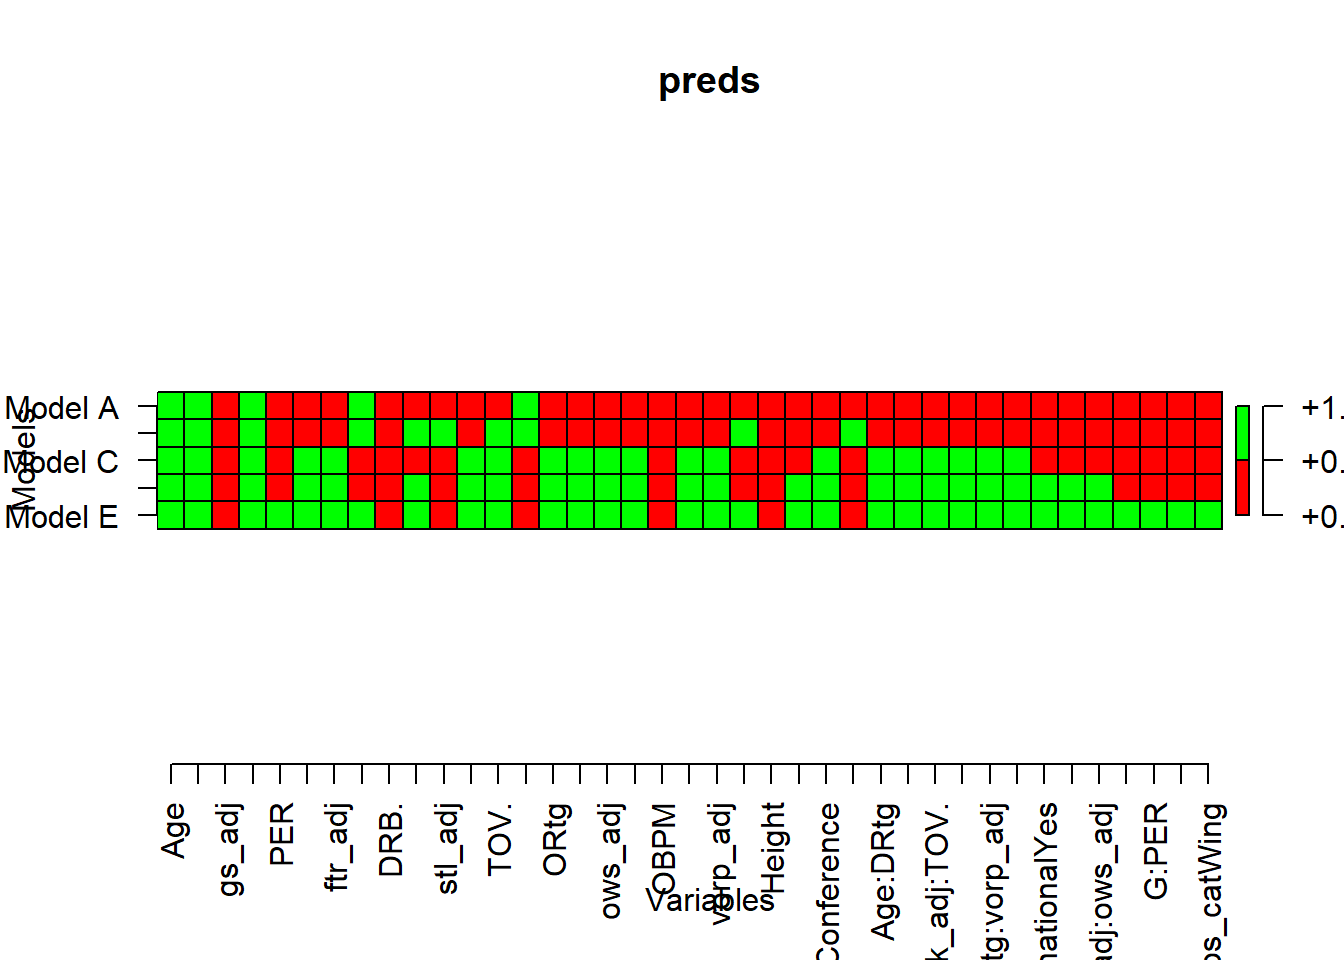
\includegraphics{FinalReportNew_files/figure-latex/unnamed-chunk-5-1.pdf}

Immediately we can see that all five proposed models use Age, G and MP
as predictors. On the other hand, none of the models use gs\_adj, DRB.,
OBPM or Height.

We'll fit each of the models and explore the residual plots.

\subsection{Residual Analysis}\label{residual-analysis}

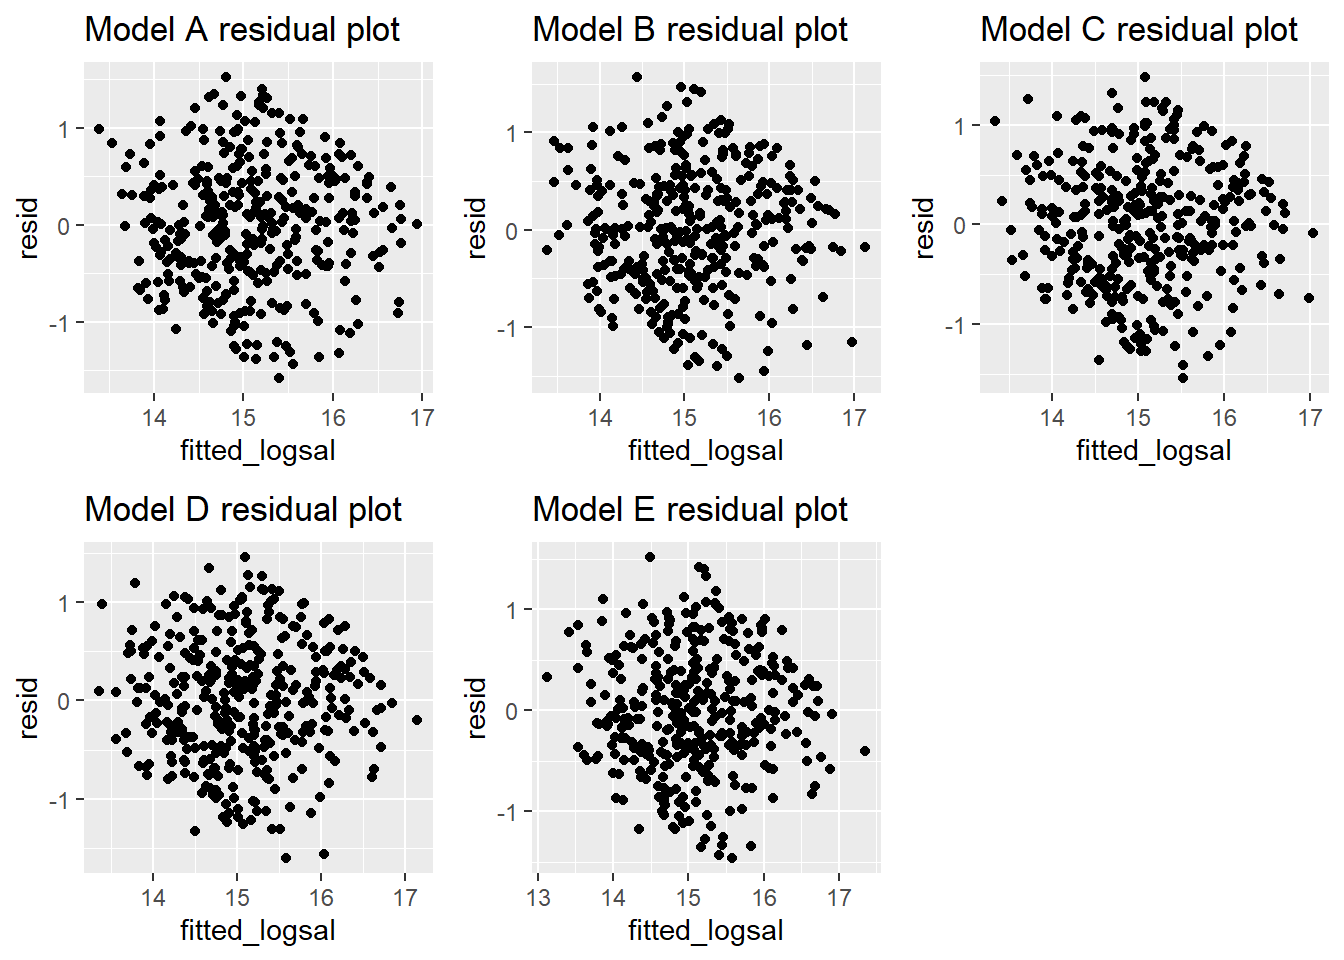
\includegraphics{FinalReportNew_files/figure-latex/p3-1.pdf}

The residual plots do not appear too problematic. However, a vague
downward trend is apparent in each and the variance is not constant
across all fitted values. Thus, these are not null plots. Fitting the
models using weighted least squares may be of interest in the future.
One persisting concern is the idea of overfitting the model. In order to
evaluate whether any of these models may be victim to overfitting or
underfitting, we'll perform 6-fold cross-validation on each model. The
number of folds is chosen to be 6 because the data has 366 observations,
so the folds will split evenly.

\subsection{Model Selection}\label{model-selection}

\begin{verbatim}
##            Model.Rsquared Model.AdjRsquared   CV.RMSE CV.Rsquared    CV.MAE
## Model A 0.561542825702464  0.55545314272611  0.638518    0.554957 0.5163634
## Model B 0.587068772936111 0.574237576614916 0.6318266   0.5665491 0.5120201
## Model C 0.587656442015736 0.562484306208557  0.642705   0.5575092 0.5264573
## Model D 0.592495638254362 0.561241616409564 0.6581126   0.5317355 0.5398083
## Model E 0.623956217060371 0.582808569079135 0.6645744   0.5348927 0.5403748
\end{verbatim}

Here, Model.Rsquared is the \(R^2\) reported by the model and
Model.AdjRsquared is the Adjusted \(R^2\) reported by the model.
Meanwhile, CV.RMSE is the average root mean squared error of the model
on unseen data from the cross-validation, CV.Rsquared is the \(R^2\) of
the model on unseen data from the cross-validation, and CV.MAE is the
mean absolute error of the model on unseen data from the
cross-validation. Ideally, we're searching for higher values for
Model.Rsquared, Model.AdjRsquared and CV.Rsquared with lower values for
CV.RMSE and CV.MAE. However, too small of a difference between model
accuracy and cross-validation accuracy may be an indication of
overfitting, while too large of a difference may be a symptom of
underfitting.

Model B performed the best in the cross-validation and we decide to
continue our analysis by considering only Model B

\subsection{Considering Weighted Least
Squares}\label{considering-weighted-least-squares}

A previously mentioned concern was the vague downward linear trend of
the residuals. We will attempt to use weighted least squares to help
resolve this. Our first attempt will involve plotting the standardized
residuals against each of the predictors as well as the inverse of each
of the predictors. This will help display if the variance in residuals
is a function of any of the individual predictors.

No clear relationship between the residuals and any predictor is
observed, so we instead use the HC3 method and compute the weights as a
function of the OLS residuals and the leverages.

\includegraphics{FinalReportNew_files/figure-latex/unnamed-chunk-10-1.pdf}

\\
\includegraphics{FinalReportNew_files/figure-latex/p5y-1.pdf}

\begin{verbatim}
## OLS:
\end{verbatim}

\begin{verbatim}
##   intercept      RMSE  Rsquared       MAE     RMSESD RsquaredSD      MAESD
## 1      TRUE 0.6347807 0.5681924 0.5134811 0.04560952  0.1059659 0.03880374
\end{verbatim}

\begin{verbatim}
## WLS:
\end{verbatim}

\begin{verbatim}
##   intercept      RMSE Rsquared       MAE     RMSESD RsquaredSD      MAESD
## 1      TRUE 0.7177479 0.448928 0.5889058 0.04701361 0.05170899 0.05281043
\end{verbatim}

We notice that the residual plot for the WLS is marginally better.
However, when evaluating each model over k-folds, the WLS performs
poorly. We suspect this is probably a case of overfitting. The OLS model
is better and it's not even close. Thus, we decided to table the WLS
idea for now.

\subsection{Model Diagnostics}\label{model-diagnostics}

In all, our model reports an \(R^2\) value of 0.5871 and Adjusted
\(R^2\) value of 0.5742. The 6-fold cross-validation procedure returns
an average \(R^2\) of 0.5665 on unseen test data, with the smallest root
mean squared error and smallest mean absolute error of any of the five
proposed models.

We will also look at the residual plot again, as well as the
standardized residual plot:

\includegraphics{FinalReportNew_files/figure-latex/p5z-1.pdf}

\\
\includegraphics{FinalReportNew_files/figure-latex/p5aa-1.pdf}

While these plots are not perfect, namely in that there appears to be a
slightly downward trend and some possible heteroscedasticity, they are
reasonable enough to suggest that none of the assumptions of the linear
model were flagrantly violated. The residuals are centered around zero,
and somewhat resemble a ``null plot.'' There does not appear to be any
significant differences between the raw and standardized residuals that
are worth discussing/exploring further.

We also looked at some of the highest leverage cases.

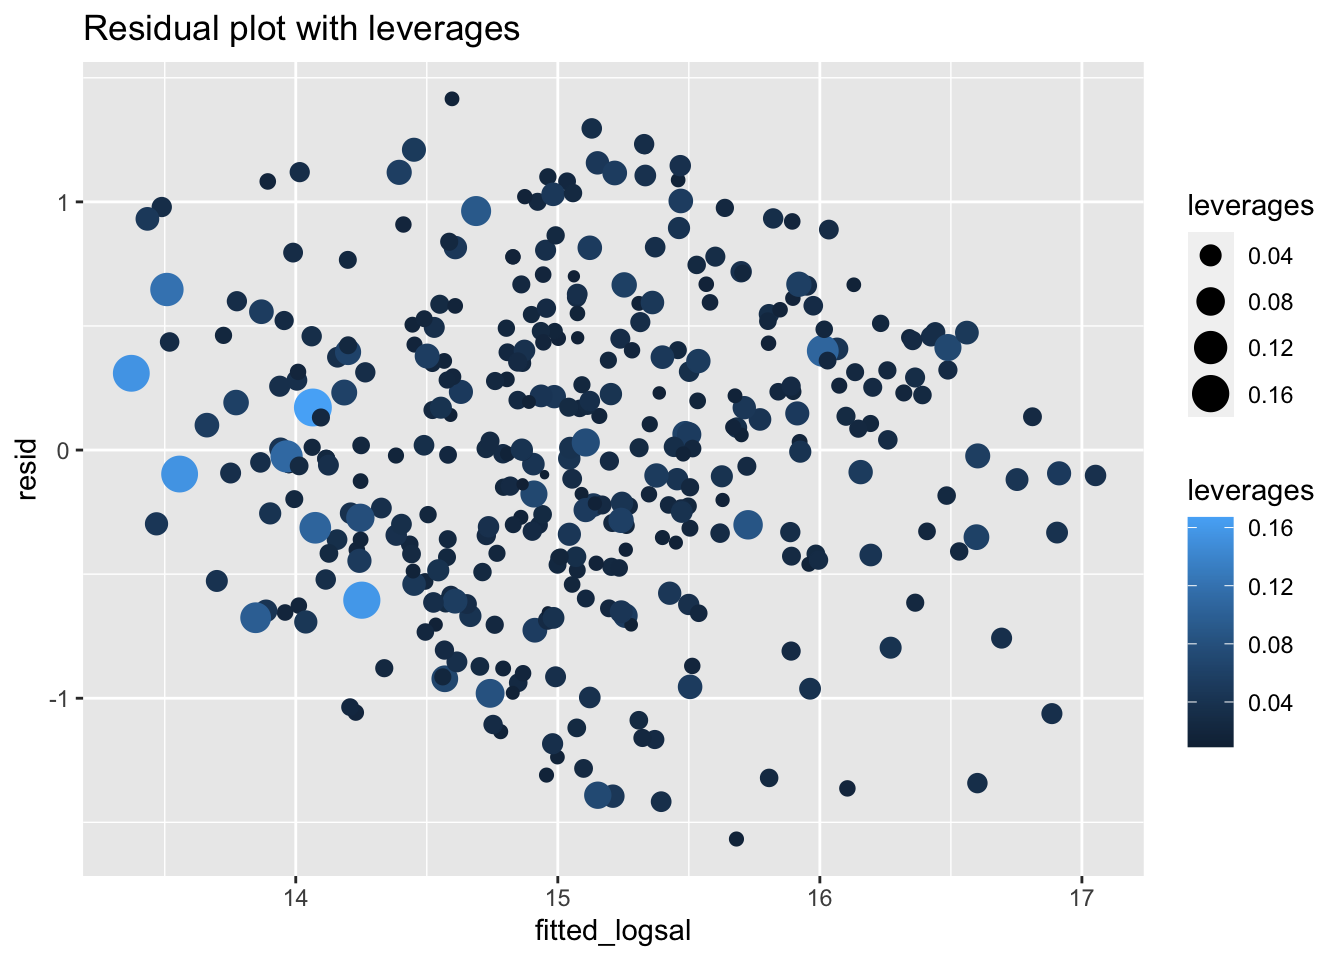
\includegraphics{FinalReportNew_files/figure-latex/p6-1.pdf}
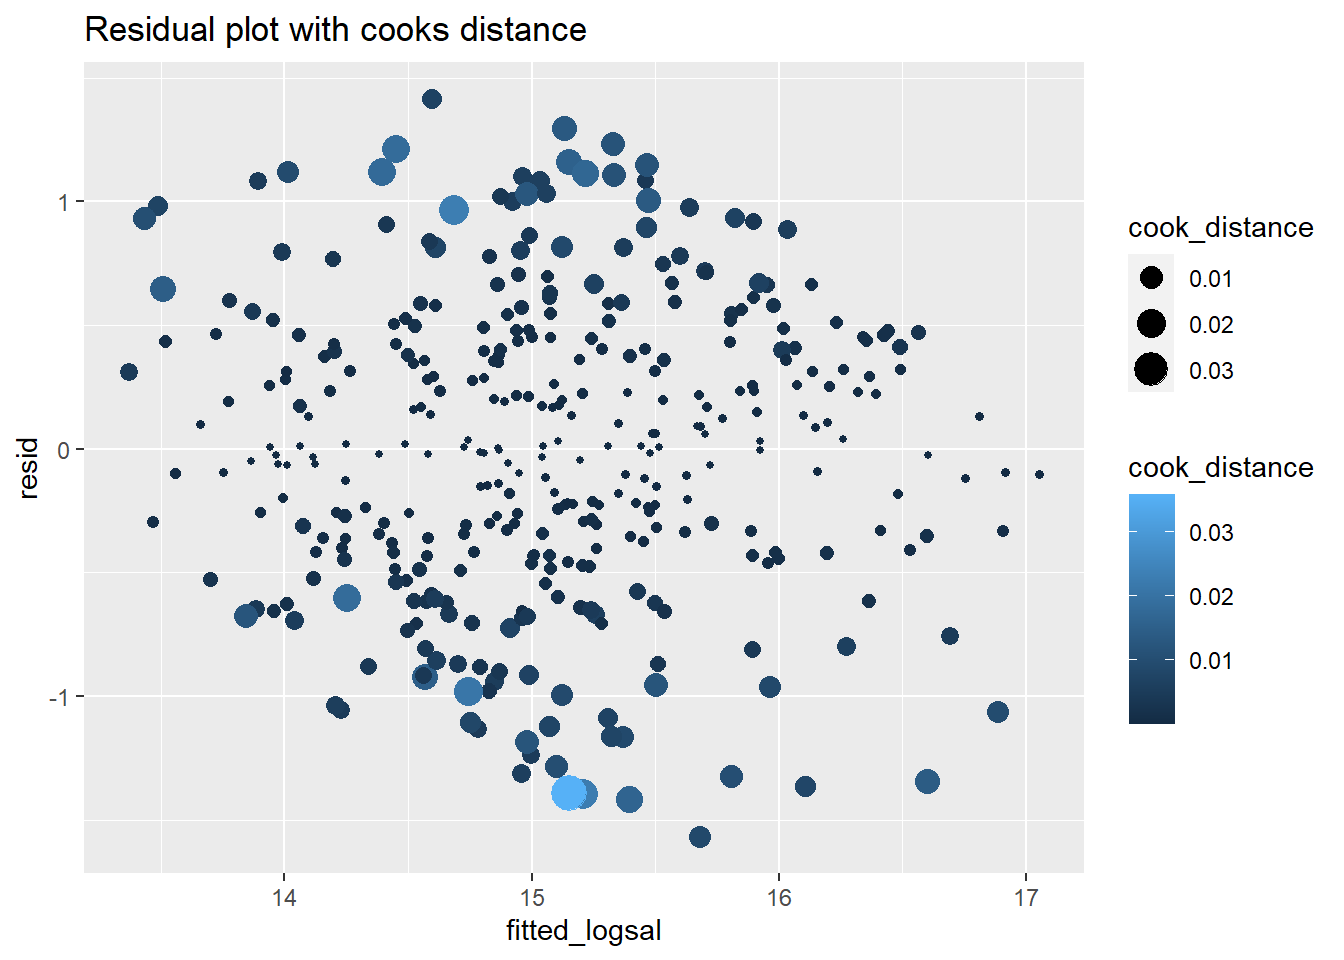
\includegraphics{FinalReportNew_files/figure-latex/p6-2.pdf}

There's an outlying case with a large leverage and Cook's Distance. The
residual does not appear to be anything extraordinary, however. After
digging into this data point, we see that it's Jarnell Stokes, a guy who
appeared in 7 games and played 18 minutes. It does appear that he has
some noisy statistics due to a small sample size from a lack of playing
time. We'll use a t-test for a mean shift to formally test if this is an
outlier.

\begin{verbatim}
## Outlier p-value:  0.04641536
\end{verbatim}

This p-value is small, but not ridiculously small in the context of a
dataset of 366 observations. We are unable to conclude that this point
is an outlier and there is a reason to believe that the mean function
for this point should be shifted.

There is another data point that is a bit of an outlier in terms of
having the largest residual. It doesn't actually appear to be an outlier
that suggests the mean function assumed by the model is incorrect,
however. This player is Iman Shumpert; we'll discuss him a bit later in
our conclusions section.

\subsection{Discussion}\label{discussion}

\subsubsection{Model Interpretation}\label{model-interpretation}

In our model, four predictors are significant at the 99.9\% confidence
level: MP, Age, G and AST. The estimated coefficients for MP, Age and
AST. are positive, which makes sense to a casual basketball fan. Players
that play more often and produce higher offensive statistics should be
paid more. Additionally, players generally tend to sign larger contracts
as their career progresses. However, G has a negative estimated
coefficient, implying that on average, players are paid less money when
they play in more games. This doesn't seem to be too logical at first.
However, one could argue that a player that plays in more games would
also generally play more minutes, and this argument would be backed by
the 0.843 correlation coefficient between these two variables in our
dataset. Perhaps one of these factors could have been removed early on,
but given they are both highly statistically significant in our final
model, it's probably good that they were both kept. The estimated
coefficients specifically for MP and for G are 0.009451 and -0.0158993,
respectively, implying that a player's predicted salary increases by
approximately 0.09\% for every extra minute played and decreases by
about 1.58\% for every extra game played. Therefore, the salary of a
player who averages 18 or more minutes a game is predicted to benefit as
the player plays more, while that of a player who averaged 17 minutes or
less per game is expected to decrease as the player plays more.

At the 99\% confidence level, two more variables are significant: USG.
And Pos\_catG. USG. has a positive estimated coefficient of 0.0244984,
indicating that a player's expected salary increases 2.48\% for every
unit increase in USG. The Pos\_catG indicator variable, conversely, has
an estimated coefficient of -0.3685353. Since this model uses
Pos\_catBig as the baseline, this model projects that a guard's
predicted salary will be more than 30\% less than a center's given that
the guard and center have identical factors for this model otherwise.

Two additional models are significant at the 90\% confidence level:
orb\_adj and stl\_adj, with a positive and negative estimated
coefficient, respectively. The idea that a player who can accumulate
more offensive rebounds is predicted to have a higher salary is
completely logical. On the other hand, a player who garners more steals
being predicted to have a lower salary may be a bit confusing for
basketball fans. A possible explanation for this could be that players
with more steals are more likely to be ``defense-first'' players, which
in 2015-16, were not as highly valued as primarily offensive skilled
players.

The estimated coefficient for the Pos\_catWing indicator variable also
becomes significant at the 90\% confidence level, with an estimated
value of -0.1741437. Like the situation for guards, our model proposes
that the predicted salary for a Wing relative to a Center with the same
model inputs otherwise is 15.98\% lower, on average. The idea that
talented bigs were much harder to come by than talented guards or wings
during this time in the NBA would be widely agreed upon by fans. This
could conceivably be why our model predicts centers with the same
model-relevant statistics as a guard or wing would have higher salaries.
Similarly, the talent pool was probably deepest among guards at this
time, so there was less of an urge to pay guards as much money.

Also present in the model are Multiteam and TOV., though neither
significant at the 90\% level. The estimated coefficient for the
Multiteam indicator variables is positive, suggesting players who played
for various teams during the 2015-16 NBA season typically had higher
salaries. The estimated coefficient for TOV. was negative, confirming
the idea that players who turned the ball over more often were paid
less, on average.

\begin{Shaded}
\begin{Highlighting}[]
\KeywordTok{summary}\NormalTok{(modB)}
\end{Highlighting}
\end{Shaded}

\begin{verbatim}
## 
## Call:
## lm(formula = logsal ~ MP + Age + USG. + G + orb_adj + AST. + 
##     stl_adj + Pos_cat + Multiteam + TOV., data = data)
## 
## Residuals:
##      Min       1Q   Median       3Q      Max 
## -1.52889 -0.41713  0.00419  0.42837  1.57068 
## 
## Coefficients:
##               Estimate Std. Error t value Pr(>|t|)    
## (Intercept) 12.5466843  0.4046700  31.005  < 2e-16 ***
## MP           0.0009451  0.0000895  10.561  < 2e-16 ***
## Age          0.0673074  0.0077536   8.681  < 2e-16 ***
## USG.         0.0244984  0.0087791   2.791 0.005547 ** 
## G           -0.0158993  0.0031515  -5.045 7.26e-07 ***
## orb_adj      0.1679352  0.0747573   2.246 0.025294 *  
## AST.         0.0220372  0.0060466   3.645 0.000308 ***
## stl_adj     -0.3190648  0.1307968  -2.439 0.015202 *  
## Pos_catG    -0.3685353  0.1394006  -2.644 0.008565 ** 
## Pos_catWing -0.1741437  0.1021098  -1.705 0.088987 .  
## Multiteam    0.1996041  0.1254847   1.591 0.112578    
## TOV.        -0.0140422  0.0089122  -1.576 0.116007    
## ---
## Signif. codes:  0 '***' 0.001 '**' 0.01 '*' 0.05 '.' 0.1 ' ' 1
## 
## Residual standard error: 0.6241 on 354 degrees of freedom
## Multiple R-squared:  0.5871, Adjusted R-squared:  0.5742 
## F-statistic: 45.75 on 11 and 354 DF,  p-value: < 2.2e-16
\end{verbatim}

\subsubsection{Contextual Applications}\label{contextual-applications}

One thing that was of interest to us was using this model to see which
players are overperforming and underperforming their salary, based on
the model's expectations. We'll look at the largest and smallest
residuals, raw and standardized:

\begin{verbatim}
## Most Underpaid: Rodney Hood, Expected Salary: 6220427, Actual Salary: 1348440
\end{verbatim}

\begin{verbatim}
## Most Overpaid: Iman Shumpert:, Expected Salary: 1868802, Actual Salary: 8988765
\end{verbatim}

Our model thought Rodney Hood was the league's most underpaid player,
and Iman Shumpert was the league's most overpaid player (using both raw
and standardized residuals, for both players). Hood's relatively high
usage rate, offensive rebounding rate, and assists led to the model
expecting him to have a fairly average salary, when he was actually paid
towards the low end of the league. Conversely, Shumpert's classification
as a guard, low usage rate and assists, and relatively high turnover
rate led the model to think he should be paid fairly low, when in
reality he was a well-paid player. We imagine that digging into which
players were over/underpaid, and whether or not this had a correlation
with team success, would be a fun and useful activity with a trustworthy
model.

\subsection{Conclusion}\label{conclusion}

In attempting to model the NBA player salary market during the 2015-16
season, we considered many variables and began by eliminating variables
we could argue wouldn't be helpful. We then proposed five models through
different methods of stepwise regression, some with interaction terms
and some with only main effects. Through the employment of k-fold
cross-validation, we decided on a best model to predict player salaries
that includes an intercept and nine main effects.

Probably the strictest limitation to our model is that it is only useful
for the 2015-16 NBA season. As the economy, the market, the player pool,
and many other factors including what assets NBA teams value in a player
change, the salary prediction model is destined to change as well.
However, even with this limitation, our model proposes not only a fun
conversation starter for basketball fans, but also a jumping off point
for future work.

With a prediction model and real data, we can investigate which players
the model deemed as overpaid and underpaid in 2015-16. Furthermore, the
question of whether overpaying players inhibits your ability to win or
whether underpaying players allows more flexibility to win can be
addressed from a team perspective.

Secondarily, we can predict what players from other eras would make in
2015-16 if they were dropped into the league with all the same
covariates. For instance, if we duplicate one of Michael Jordan's
greatest seasons as a 2015-16 performance, we can predict what Jordan's
salary may have been. Comparing our model's prediction to his actual
salary under the consideration of inflation may support the discussion
regarding how quickly and drastically NBA contracts are growing.
Performing this type of analysis over a larger group of players could
also provide insight to how the values of NBA teams have changed over
time by investigating which predictors are more significant in different
eras of basketball.

Most importantly, our work provides a notion of how to develop such a
model. Despite the limitation mentioned prior, one could use the methods
outlined in this paper to construct a similar model for another season,
with different potential covariates, or even for an entirely different
sport.

Any future advancement of this work should, however, consider the idea
of holding out a test set until the very end of the model construction.
Such a decision may have provided more validation for our model had we
chosen to do so.

\newpage

\subsection{Appendix}\label{appendix}

\paragraph{Figure A1: Transformation of
VORP}\label{figure-a1-transformation-of-vorp}

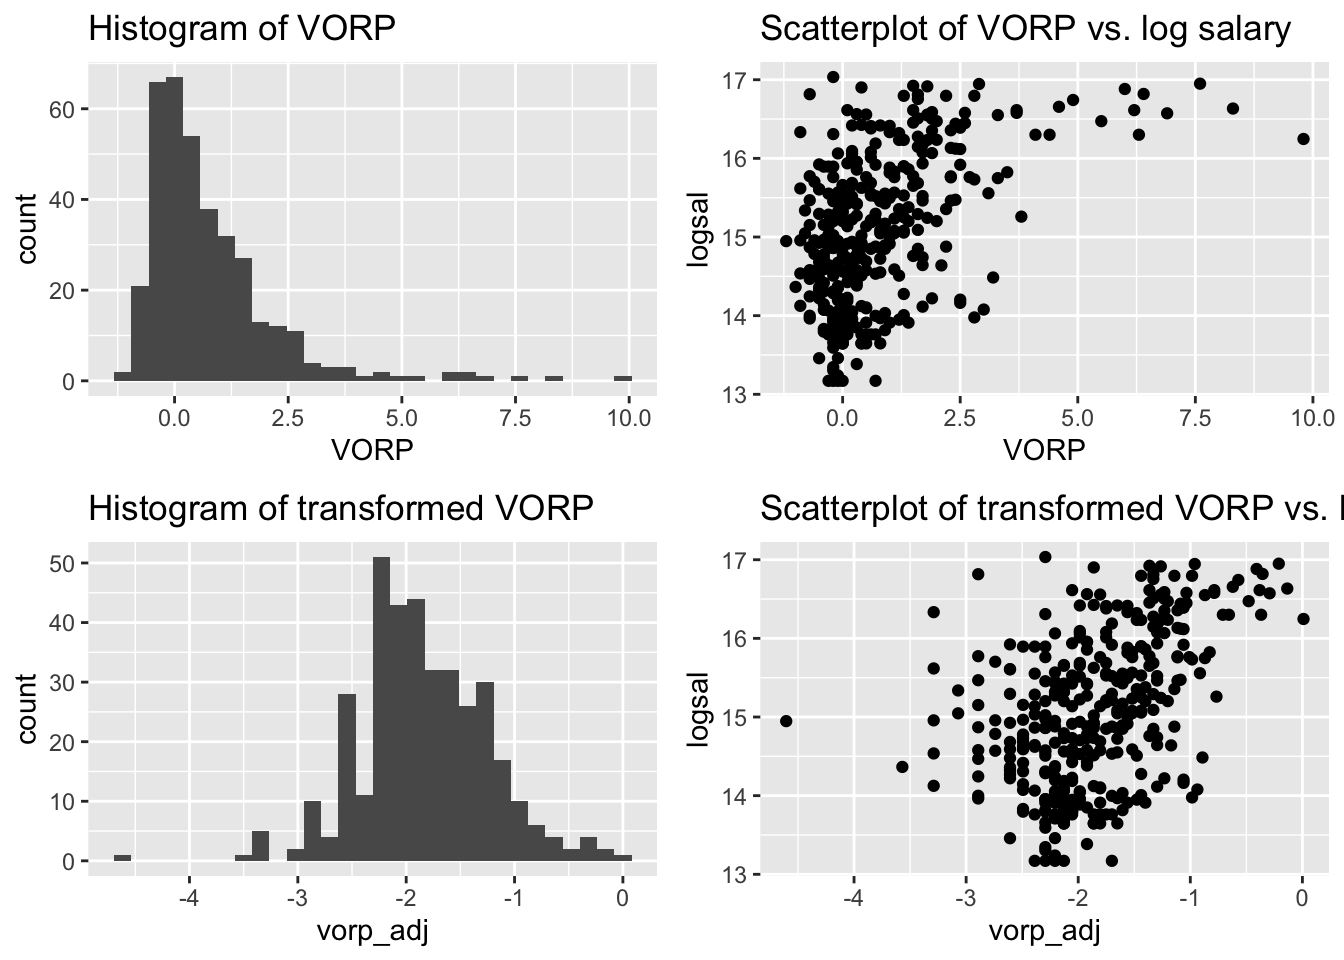
\includegraphics{FinalReportNew_files/figure-latex/p0-1.pdf}

\paragraph{Figure A2: Transformation of
Pos}\label{figure-a2-transformation-of-pos}

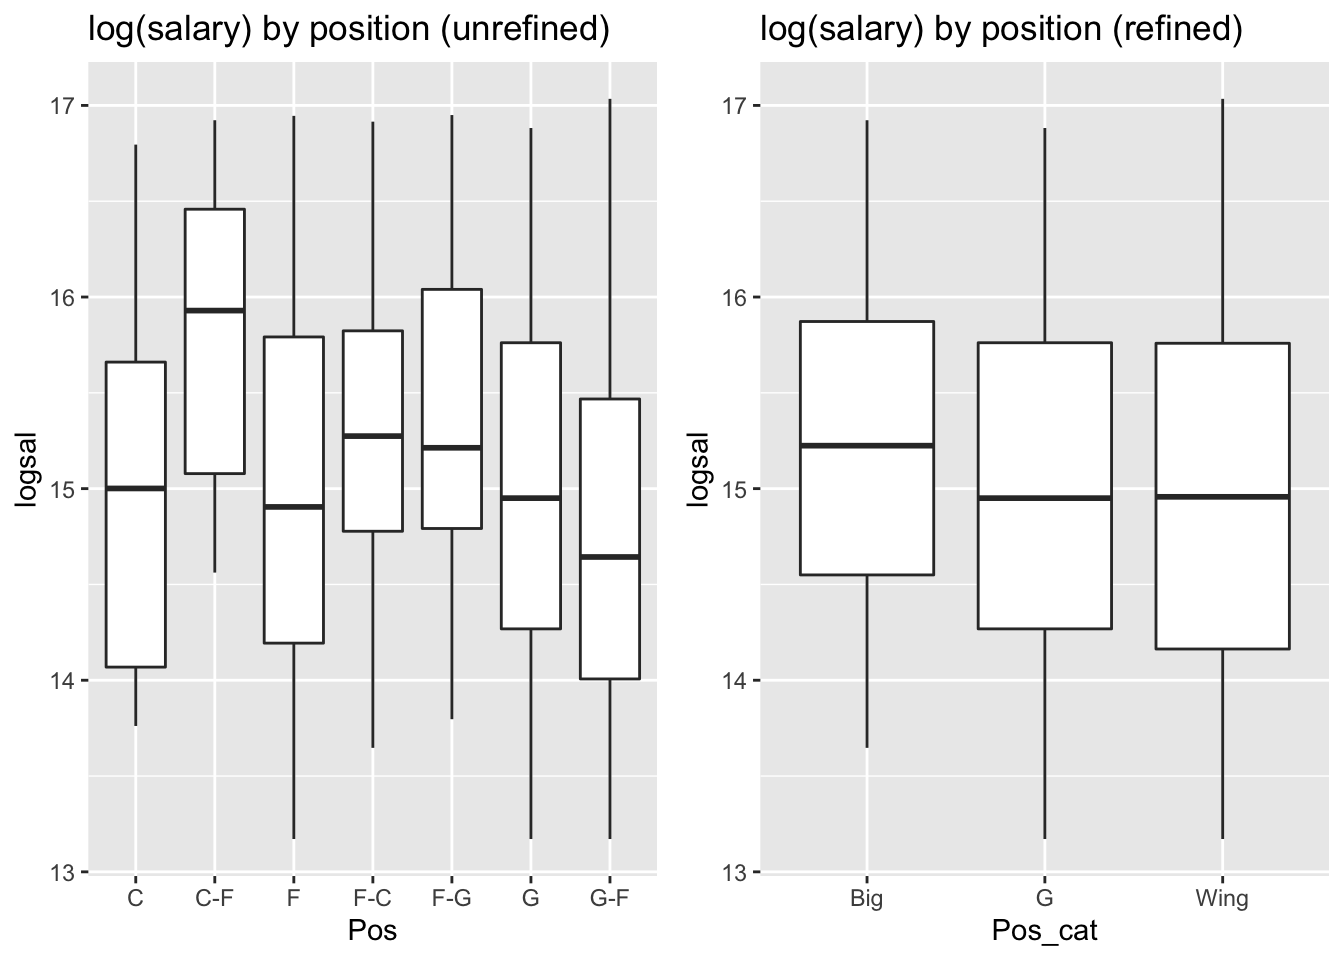
\includegraphics{FinalReportNew_files/figure-latex/p2b-1.pdf}

\paragraph{Output A3: Summaries of Models A, C, D,
E}\label{output-a3-summaries-of-models-a-c-d-e}

\begin{Shaded}
\begin{Highlighting}[]
\KeywordTok{summary}\NormalTok{(modA)}
\end{Highlighting}
\end{Shaded}

\begin{verbatim}
## 
## Call:
## lm(formula = logsal ~ MP + Age + USG. + G + orb_adj, data = data)
## 
## Residuals:
##      Min       1Q   Median       3Q      Max 
## -1.58284 -0.42013  0.01819  0.44269  1.52349 
## 
## Coefficients:
##               Estimate Std. Error t value Pr(>|t|)    
## (Intercept)  1.149e+01  2.983e-01  38.537  < 2e-16 ***
## MP           9.743e-04  8.853e-05  11.005  < 2e-16 ***
## Age          7.777e-02  7.573e-03  10.269  < 2e-16 ***
## USG.         3.904e-02  7.685e-03   5.080 6.06e-07 ***
## G           -1.632e-02  3.189e-03  -5.120 4.99e-07 ***
## orb_adj      2.360e-01  5.318e-02   4.438 1.21e-05 ***
## ---
## Signif. codes:  0 '***' 0.001 '**' 0.01 '*' 0.05 '.' 0.1 ' ' 1
## 
## Residual standard error: 0.6378 on 360 degrees of freedom
## Multiple R-squared:  0.5615, Adjusted R-squared:  0.5555 
## F-statistic: 92.21 on 5 and 360 DF,  p-value: < 2.2e-16
\end{verbatim}

\begin{Shaded}
\begin{Highlighting}[]
\KeywordTok{summary}\NormalTok{(modC)}
\end{Highlighting}
\end{Shaded}

\begin{verbatim}
## 
## Call:
## lm(formula = logsal ~ Age + G + MP + X3PAr + ftr_adj + blk_adj + 
##     TOV. + ORtg + DRtg + ows_adj + dws_adj + OBPM + DBPM + Conference + 
##     Multiteam + Age:DRtg + G:ftr_adj + ORtg:DBPM + DRtg:vorp_adj + 
##     dws_adj:Conference, data = data)
## 
## Residuals:
##      Min       1Q   Median       3Q      Max 
## -1.54700 -0.43076  0.00133  0.43552  1.48162 
## 
## Coefficients: (1 not defined because of singularities)
##                           Estimate Std. Error t value Pr(>|t|)    
## (Intercept)             24.3370946  5.7889365   4.204 3.35e-05 ***
## Age                     -0.3634540  0.2010862  -1.807 0.071565 .  
## G                       -0.0205188  0.0058113  -3.531 0.000471 ***
## MP                       0.0007349  0.0001368   5.371 1.44e-07 ***
## X3PAr                   -0.9804816  0.2545241  -3.852 0.000140 ***
## ftr_adj                  0.0907917  0.4787728   0.190 0.849708    
## blk_adj                  0.1317285  0.1070956   1.230 0.219534    
## TOV.                     0.0024759  0.0091792   0.270 0.787527    
## ORtg                    -0.0136113  0.0061828  -2.201 0.028365 *  
## DRtg                    -0.0943876  0.0546363  -1.728 0.084964 .  
## ows_adj                  0.6398036  0.3231635   1.980 0.048521 *  
## dws_adj                  0.7796038  0.2527172   3.085 0.002201 ** 
## OBPM                     0.1075956  0.0325159   3.309 0.001035 ** 
## DBPM                    -0.1172800  0.1658451  -0.707 0.479942    
## ConferenceMulti         -0.6154735  0.3140875  -1.960 0.050854 .  
## ConferenceWest          -0.0399846  0.1719007  -0.233 0.816208    
## Multiteam                       NA         NA      NA       NA    
## Age:DRtg                 0.0040700  0.0018897   2.154 0.031958 *  
## G:ftr_adj               -0.0083647  0.0091081  -0.918 0.359062    
## ORtg:DBPM                0.0006980  0.0015070   0.463 0.643528    
## DRtg:vorp_adj           -0.0038339  0.0014272  -2.686 0.007576 ** 
## dws_adj:ConferenceMulti  0.8014378  0.3168241   2.530 0.011865 *  
## dws_adj:ConferenceWest   0.0122395  0.1417901   0.086 0.931261    
## ---
## Signif. codes:  0 '***' 0.001 '**' 0.01 '*' 0.05 '.' 0.1 ' ' 1
## 
## Residual standard error: 0.6327 on 344 degrees of freedom
## Multiple R-squared:  0.5877, Adjusted R-squared:  0.5625 
## F-statistic: 23.35 on 21 and 344 DF,  p-value: < 2.2e-16
\end{verbatim}

\begin{Shaded}
\begin{Highlighting}[]
\KeywordTok{summary}\NormalTok{(modD)}
\end{Highlighting}
\end{Shaded}

\begin{verbatim}
## 
## Call:
## lm(formula = logsal ~ Age + G + MP + X3PAr + ftr_adj + blk_adj + 
##     TOV. + ORtg + DRtg + ows_adj + dws_adj + OBPM + DBPM + Conference + 
##     Multiteam + Age:DRtg + G:ftr_adj + ORtg:DBPM + DRtg:vorp_adj + 
##     dws_adj:Conference + AST. + International + Age:International + 
##     AST.:vorp_adj + blk_adj:ows_adj, data = data)
## 
## Residuals:
##      Min       1Q   Median       3Q      Max 
## -1.60508 -0.41357 -0.00006  0.44588  1.46092 
## 
## Coefficients: (1 not defined because of singularities)
##                           Estimate Std. Error t value Pr(>|t|)    
## (Intercept)             22.2370339  5.9249408   3.753 0.000205 ***
## Age                     -0.3178714  0.2059278  -1.544 0.123617    
## G                       -0.0195414  0.0058950  -3.315 0.001016 ** 
## MP                       0.0007410  0.0001392   5.324 1.85e-07 ***
## X3PAr                   -0.8983312  0.2732157  -3.288 0.001115 ** 
## ftr_adj                  0.1248435  0.4828380   0.259 0.796130    
## blk_adj                  0.6152379  0.3401905   1.809 0.071413 .  
## TOV.                    -0.0051613  0.0110587  -0.467 0.641001    
## ORtg                    -0.0120686  0.0069953  -1.725 0.085392 .  
## DRtg                    -0.0816310  0.0555805  -1.469 0.142842    
## ows_adj                  0.2684077  0.4355453   0.616 0.538139    
## dws_adj                  0.7393603  0.2558302   2.890 0.004100 ** 
## OBPM                     0.0881014  0.0410655   2.145 0.032632 *  
## DBPM                    -0.0073067  0.1757420  -0.042 0.966861    
## ConferenceMulti         -0.5774061  0.3202062  -1.803 0.072240 .  
## ConferenceWest          -0.0276285  0.1727601  -0.160 0.873036    
## Multiteam                       NA         NA      NA       NA    
## AST.                     0.0115624  0.0115038   1.005 0.315571    
## InternationalYes         0.3711941  0.4903642   0.757 0.449590    
## Age:DRtg                 0.0036654  0.0019291   1.900 0.058272 .  
## G:ftr_adj               -0.0094222  0.0093016  -1.013 0.311795    
## ORtg:DBPM               -0.0002576  0.0015912  -0.162 0.871488    
## DRtg:vorp_adj           -0.0041319  0.0015758  -2.622 0.009135 ** 
## dws_adj:ConferenceMulti  0.7790781  0.3212554   2.425 0.015826 *  
## dws_adj:ConferenceWest   0.0055229  0.1427027   0.039 0.969150    
## Age:InternationalYes    -0.0109916  0.0182472  -0.602 0.547328    
## vorp_adj:AST.            0.0031188  0.0057195   0.545 0.585907    
## blk_adj:ows_adj          0.4499859  0.3071171   1.465 0.143795    
## ---
## Signif. codes:  0 '***' 0.001 '**' 0.01 '*' 0.05 '.' 0.1 ' ' 1
## 
## Residual standard error: 0.6336 on 339 degrees of freedom
## Multiple R-squared:  0.5925, Adjusted R-squared:  0.5612 
## F-statistic: 18.96 on 26 and 339 DF,  p-value: < 2.2e-16
\end{verbatim}

\begin{Shaded}
\begin{Highlighting}[]
\KeywordTok{summary}\NormalTok{(modE)}
\end{Highlighting}
\end{Shaded}

\begin{verbatim}
## 
## Call:
## lm(formula = logsal ~ Age + G + MP + X3PAr + ftr_adj + blk_adj + 
##     TOV. + ORtg + DRtg + ows_adj + dws_adj + OBPM + DBPM + Conference + 
##     Multiteam + Age:DRtg + G:ftr_adj + ORtg:DBPM + DRtg:vorp_adj + 
##     dws_adj:Conference + AST. + International + Age:International + 
##     AST.:vorp_adj + blk_adj:ows_adj + orb_adj + Pos_cat + Age:ows_adj + 
##     G:PER + PER + ftr_adj:Pos_cat + orb_adj:Pos_cat, data = data)
## 
## Residuals:
##      Min       1Q   Median       3Q      Max 
## -1.46394 -0.38934 -0.01977  0.42035  1.52098 
## 
## Coefficients: (1 not defined because of singularities)
##                           Estimate Std. Error t value Pr(>|t|)    
## (Intercept)             27.3909654  6.3043721   4.345 1.86e-05 ***
## Age                     -0.3068498  0.2037641  -1.506  0.13305    
## G                       -0.0126248  0.0081698  -1.545  0.12324    
## MP                       0.0008406  0.0001439   5.840 1.25e-08 ***
## X3PAr                   -0.6860913  0.3917484  -1.751  0.08082 .  
## ftr_adj                 -0.8792976  0.8476363  -1.037  0.30033    
## blk_adj                  0.5726771  0.3705746   1.545  0.12322    
## TOV.                    -0.0147863  0.0116375  -1.271  0.20478    
## ORtg                    -0.0194670  0.0085058  -2.289  0.02273 *  
## DRtg                    -0.1261219  0.0586503  -2.150  0.03225 *  
## ows_adj                 -0.7792757  0.9717120  -0.802  0.42315    
## dws_adj                  0.5833818  0.2551673   2.286  0.02287 *  
## OBPM                     0.1469162  0.0560501   2.621  0.00917 ** 
## DBPM                    -0.2860053  0.2003910  -1.427  0.15446    
## ConferenceMulti         -0.5006344  0.3248737  -1.541  0.12428    
## ConferenceWest          -0.0868621  0.1706016  -0.509  0.61099    
## Multiteam                       NA         NA      NA       NA    
## AST.                     0.0196097  0.0119977   1.634  0.10312    
## InternationalYes         0.3513921  0.4976175   0.706  0.48060    
## orb_adj                  0.2303645  0.2586614   0.891  0.37379    
## Pos_catG                -1.0450298  0.5797196  -1.803  0.07236 .  
## Pos_catWing             -0.9649262  0.5573017  -1.731  0.08431 .  
## PER                     -0.0057340  0.0406040  -0.141  0.88779    
## Age:DRtg                 0.0041170  0.0019414   2.121  0.03470 *  
## G:ftr_adj               -0.0029518  0.0100943  -0.292  0.77015    
## ORtg:DBPM                0.0018014  0.0018211   0.989  0.32329    
## DRtg:vorp_adj           -0.0037921  0.0015821  -2.397  0.01709 *  
## dws_adj:ConferenceMulti  0.6797103  0.3233676   2.102  0.03632 *  
## dws_adj:ConferenceWest   0.0636803  0.1406019   0.453  0.65091    
## Age:InternationalYes    -0.0125764  0.0184709  -0.681  0.49643    
## vorp_adj:AST.           -0.0016345  0.0057887  -0.282  0.77784    
## blk_adj:ows_adj          0.4048766  0.3091624   1.310  0.19125    
## Age:ows_adj              0.0578625  0.0322263   1.796  0.07349 .  
## G:PER                   -0.0009189  0.0005754  -1.597  0.11120    
## ftr_adj:Pos_catG         1.1163576  0.7707307   1.448  0.14845    
## ftr_adj:Pos_catWing      1.2413983  0.7491820   1.657  0.09847 .  
## orb_adj:Pos_catG        -0.0339494  0.3022905  -0.112  0.91065    
## orb_adj:Pos_catWing      0.0216544  0.2592782   0.084  0.93349    
## ---
## Signif. codes:  0 '***' 0.001 '**' 0.01 '*' 0.05 '.' 0.1 ' ' 1
## 
## Residual standard error: 0.6178 on 329 degrees of freedom
## Multiple R-squared:  0.624,  Adjusted R-squared:  0.5828 
## F-statistic: 15.16 on 36 and 329 DF,  p-value: < 2.2e-16
\end{verbatim}

\end{document}
